

\section{Simple Shapes}


   \begin{figure}[h!]

     \centering
        
        \begin{subfigure}[b]{0.45\textwidth}
          
\includegraphics[width=\textwidth]{circle.png}
          \caption{Circle}
          \label{fig:circle}
        \end{subfigure}
        \hfill
        \begin{subfigure}[b]{0.45\textwidth}
          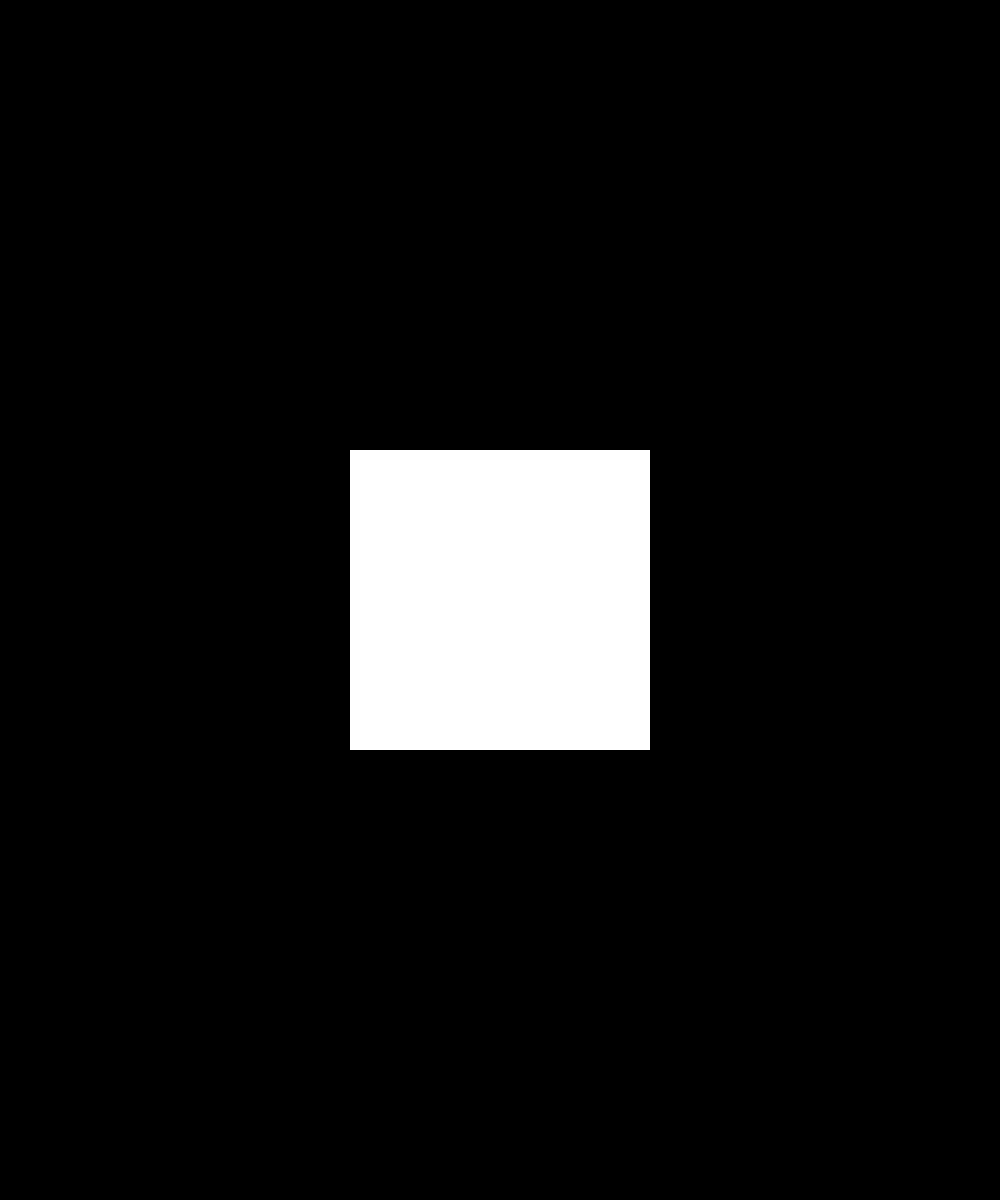
\includegraphics[width=\textwidth]{rectangle.png}
          \caption{Rectangle}
          \label{fig:rectangle}
        \end{subfigure}

        \caption{Each image size is $1200$ by $1000$ pixels with
          $90000$ white pixels.}
        \label{fig:simple_imgs}

   \end{figure}
   



\section{Complicated Branching Structures}

   
    \begin{figure}

     \centering
        
        \begin{subfigure}[b]{0.45\textwidth}
          
\includegraphics[width=\textwidth]{G_1_L_3.png}
          \caption{$G_1L_3$}
          \label{fig:G1L3}
        \end{subfigure}
        \hfill
        \begin{subfigure}[b]{0.45\textwidth}
          
\includegraphics[width=\textwidth]{G_1_L_4.png}
          \caption{$G_1L_4$}
          \label{fig:G1L4}
        \end{subfigure}

        \begin{subfigure}[b]{0.45\textwidth}
          
\includegraphics[width=\textwidth]{G_1_L_5.png}
          \caption{$G_1L_5$}
          \label{fig:G1L5}
        \end{subfigure}
        \hfill
        \begin{subfigure}[b]{0.45\textwidth}
          
\includegraphics[width=\textwidth]{G_1_L_6.png}
          \caption{$G_1L_6$}
          \label{fig:G1L6}
        \end{subfigure}

        \caption{In the group one, each image size is $1200$ by $1000$ pixels with
          $90000$ white pixels.}
        \label{fig:G1_imgs}

    \end{figure}




    \begin{figure}

     \centering
        
        \begin{subfigure}[b]{0.45\textwidth}
          
\includegraphics[width=\textwidth]{G_2_L_3.png}
          \caption{$G_2L_3$}
          \label{fig:G2L3}
        \end{subfigure}
        \hfill
        \begin{subfigure}[b]{0.45\textwidth}
          
\includegraphics[width=\textwidth]{G_2_L_4.png}
          \caption{$G_2L_4$}
          \label{fig:G2L4}
        \end{subfigure}

        \begin{subfigure}[b]{0.45\textwidth}
          
\includegraphics[width=\textwidth]{G_2_L_5.png}
          \caption{$G_2L_5$}
          \label{fig:G2L5}
        \end{subfigure}
        \hfill
        \begin{subfigure}[b]{0.45\textwidth}
          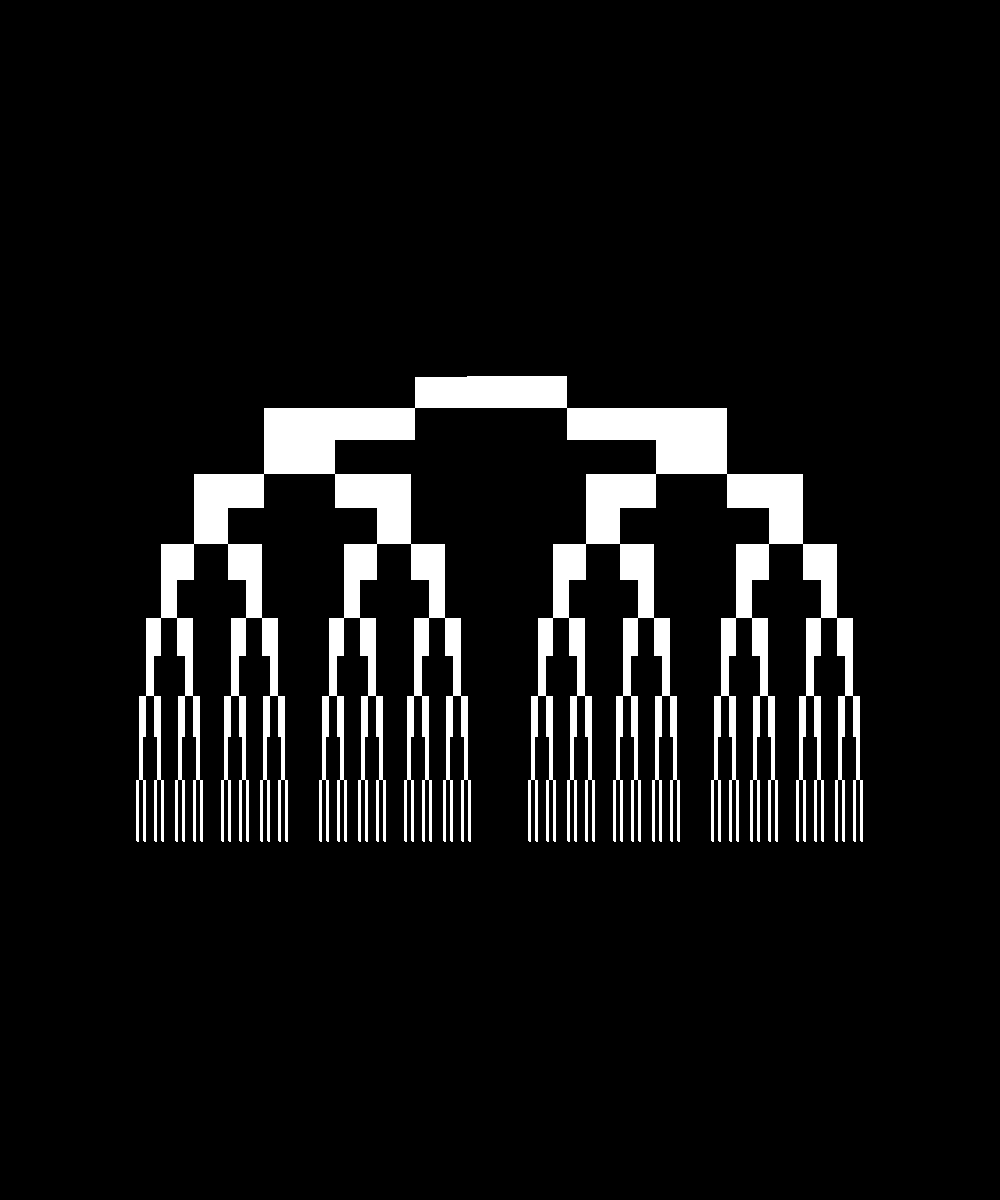
\includegraphics[width=\textwidth]{G_2_L_6.png}
          \caption{$G_2L_6$}
          \label{fig:G2L6}
        \end{subfigure}

        \caption{In the group two, each image size is $1200$ by $1000$ pixels with
          $90000$ white pixels.}
        \label{fig:G2_imgs}

   \end{figure}
